
\chapter{实验测试与结果分析}

\section{实验环境与测试负载}

\subsection{实验环境}

本研究涉及对Linux内核的深度修改与定制,实验环境的选择受到多种因素的限制。首先,由于对内核进行了大量底层改动,测试环境需要完全控制系统底层权限并能够频繁重启以更新内核,而生产环境不允许此类操作;其次,修改后的内核需要经过充分验证才能部署到高端服务器上,以避免潜在的系统稳定性问题。因此,本研究采用了性能较为有限的笔记本电脑作为测试平台,虽然测试平台的绝对性能与企业级服务器存在差距,但本研究关注的是不同算法间的相对性能比较,以及算法在不同工作负载下的适应性表现,这些方面的结论在很大程度上可以推广到更高性能的硬件环境中。未来研究中,在核心算法稳定后,可考虑在大规模服务器集群上进行进一步验证。

\begin{table}[ht]
    \centering
    \caption{实验平台硬件配置}
    \label{tab:hardware_config}
    \begin{tabular}{ll}
        \toprule
        CPU & Intel(R) Core(TM) i7-8750H @ 2.20GHz \\
        \midrule
        Memory & 16GB (2 \(\times\) 8GB) DDR4 @ 2667MT/s SODIMM \\
        \midrule
        SSD & Intel SSDPEKKW256G8 NVMe SSD (256GB, PCIe Gen3 x4)  \\
        \midrule
        HDD & Seagate ST1000LM035 HDD (1TB, 5400 RPM) \\
        \bottomrule
    \end{tabular}
\end{table}
表\ref{tab:hardware_config}汇总了实验平台的具体配置,可以看到该平台拥有 Intel(R) Core(TM) i7-8750H CPU @ 2.20GHz 以及 16GB DDR4 内存。为了在内核中进行对比,本研究分别选取了机械硬盘、SSD 和 ZRAM 这三种不同的卸载后端。之所以进行这样的选择,一方面是由于官方内核暂未实现基于 RDMA 和 NVM 的卸载后端,另一方面也是为了更好地体现不同存储介质在 I/O 延迟和读写性能方面的差异。机械硬盘能够代表最传统、也是性能相对最差的卸载方式,SSD 在随机读写和延迟方面有一定程度提升,而 ZRAM 则具有数据压缩和低延迟的优势,通常被认为是内存交换的优先方案。为了凸显 ZRAM 的潜在优势,并评估自适应算法在高压缩比数据下的实际效果,本文在后续测试中也将 ZRAM 视为可获得最优 I/O 性能的后端加以重点分析。


\subsection{测试负载}

在负载选择方面,为了更全面地测试本文提出方案的通用性,实验分别使用了文件密集型的 Web Server 和内存密集型的 Redis 这两类典型应用。Web Server 场景主要用于观察系统针对大量静态文件(包括高清图片与文本数据)缓存时的文件页回收策略,而 Redis 场景则聚焦在匿名页占比极高的内存回收状态。

对于 Web Server 负载,为了实现文件密集型操作,测试系统使用了图床服务作为测试对象。图床服务需要处理大量的静态文件,包括高清图片和文本数据,这些文件的访问模式具有明显的文件密集型特征。并且系统实现了限流器,一旦请求延迟超过100ms,则停止服务新的请求,通过这种方式可以使用每秒请求数(Request Per Second,RPS)来衡量系统的性能。

值得注意的是,在 Redis 测试中禁止了持久化功能并关闭了淘汰策略,这样能更直接地暴露内存回收在内核层面的有效性,因为一旦允许用户态自行管理持久化或淘汰,就会在应用层与内核层产生额外耦合,从而干扰对回收策略的评估。



\section{模块功能与有效性测试}

\subsection{内存压力模块有效性验证}


\begin{figure}[htb]
    \centering
    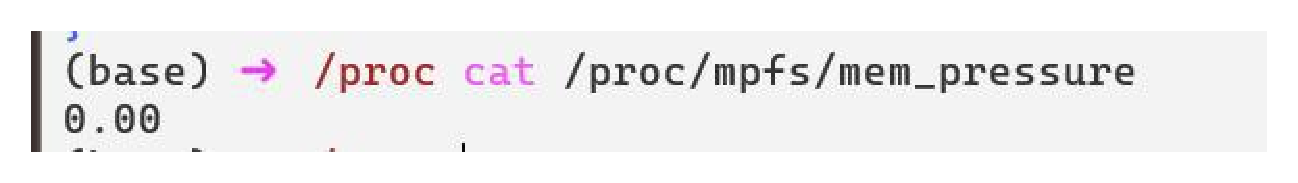
\includegraphics[width=\textwidth,keepaspectratio]{proc_mem_press.pdf}
    \caption{获取内存压力的接口}
    \label{fig:proc_mem_press}
\end{figure}

为验证内存压力模块能否在相同负载条件下,针对不同存储后端生成准确的内存压力测量值,测试系统设计了一个 Web 服务器基准测试。测试在服务器端预先加载了各类图片和文本文件,随后利用压力发生器持续随机发起请求。在内核层面,分别配置了三种不同的存储后端用于内存卸载:传统机械硬盘、SSD和 ZRAM。

\begin{figure}[htb]
    \centering
    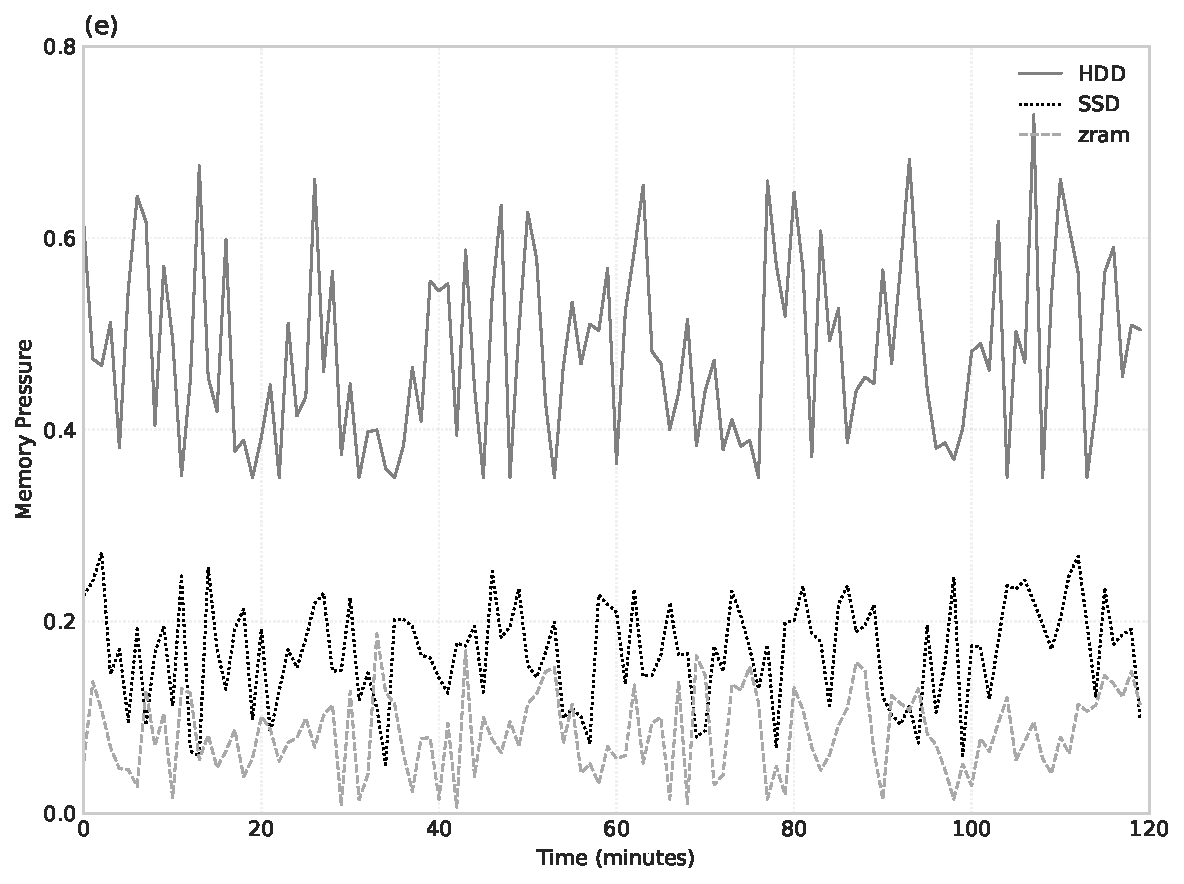
\includegraphics[width=\textwidth,keepaspectratio]{memory_pressure.pdf}
    \caption{三种卸载后端下的内存压力对比}
    \label{fig:memory_pressure}
\end{figure}
该实验以系统可用内存从 16GB 开始,逐步降低至 6GB,此时基于机械硬盘的配置已无法正常工作。通过这种方法,进行多轮测试,并观察系统在不同存储后端下对内存压力的响应情况。测试通过一个脚本,每 1 分钟通过如图\ref{fig:proc_mem_press}所示的接口获取系统内存压力。

图\ref{fig:memory_pressure}展示了三种卸载后端在 120 分钟时间段内的内存压力曲线。结果清晰地显示了系统行为的差异:
\begin{itemize}
    \item 机械硬盘(实线):由于读写延迟和带宽的限制,机械硬盘配置频繁触发页面换入换出操作。这导致系统大量时间处于高压力状态($0.4$-$0.7$ 范围),难以为传入请求维持稳定服务。
    \item SSD(点线):凭借更快的 I/O 响应能力,SSD 维持了明显较低的内存压力(约 $0.1$-$0.25$ 范围),相较于机械硬盘配置表现出显著改善。
    \item ZRAM(虚线):利用压缩和低访问延迟的双重优势,ZRAM 表现最佳,内存压力读数最低(通常低于 $0.15$),有效缓解了内存压力峰值。
\end{itemize}

通过该实验可以确认本研究的内存压力模块在不同后端下均能触发与还原高压场景所需的换页流程,且能够准确地量化系统内存使用状况,为后续的自适应回收算法测试奠定基础。


\subsection{文件页与匿名页均衡算法有效性验证}
\label{sec:file_page_anonymous_page_balance_algorithm_validation}

在确认内存压力模块可以生成可控且真实的压力环境后,需要检验自适应回收算法的第二个核心:即针对文件页与匿名页的均衡回收机制。为此,本文选取了 10GB 的可用内存作为上限来运行高负载场景,并针对 Linux 内核中的\(swappiness\)参数进行多轮对比测试。实验中分别测试了使用默认内核策略(baseline)和启用自适应均衡算法(adaptive swappiness)两种情况下的系统性能表现。

\begin{figure}[htbp]
    \centering
    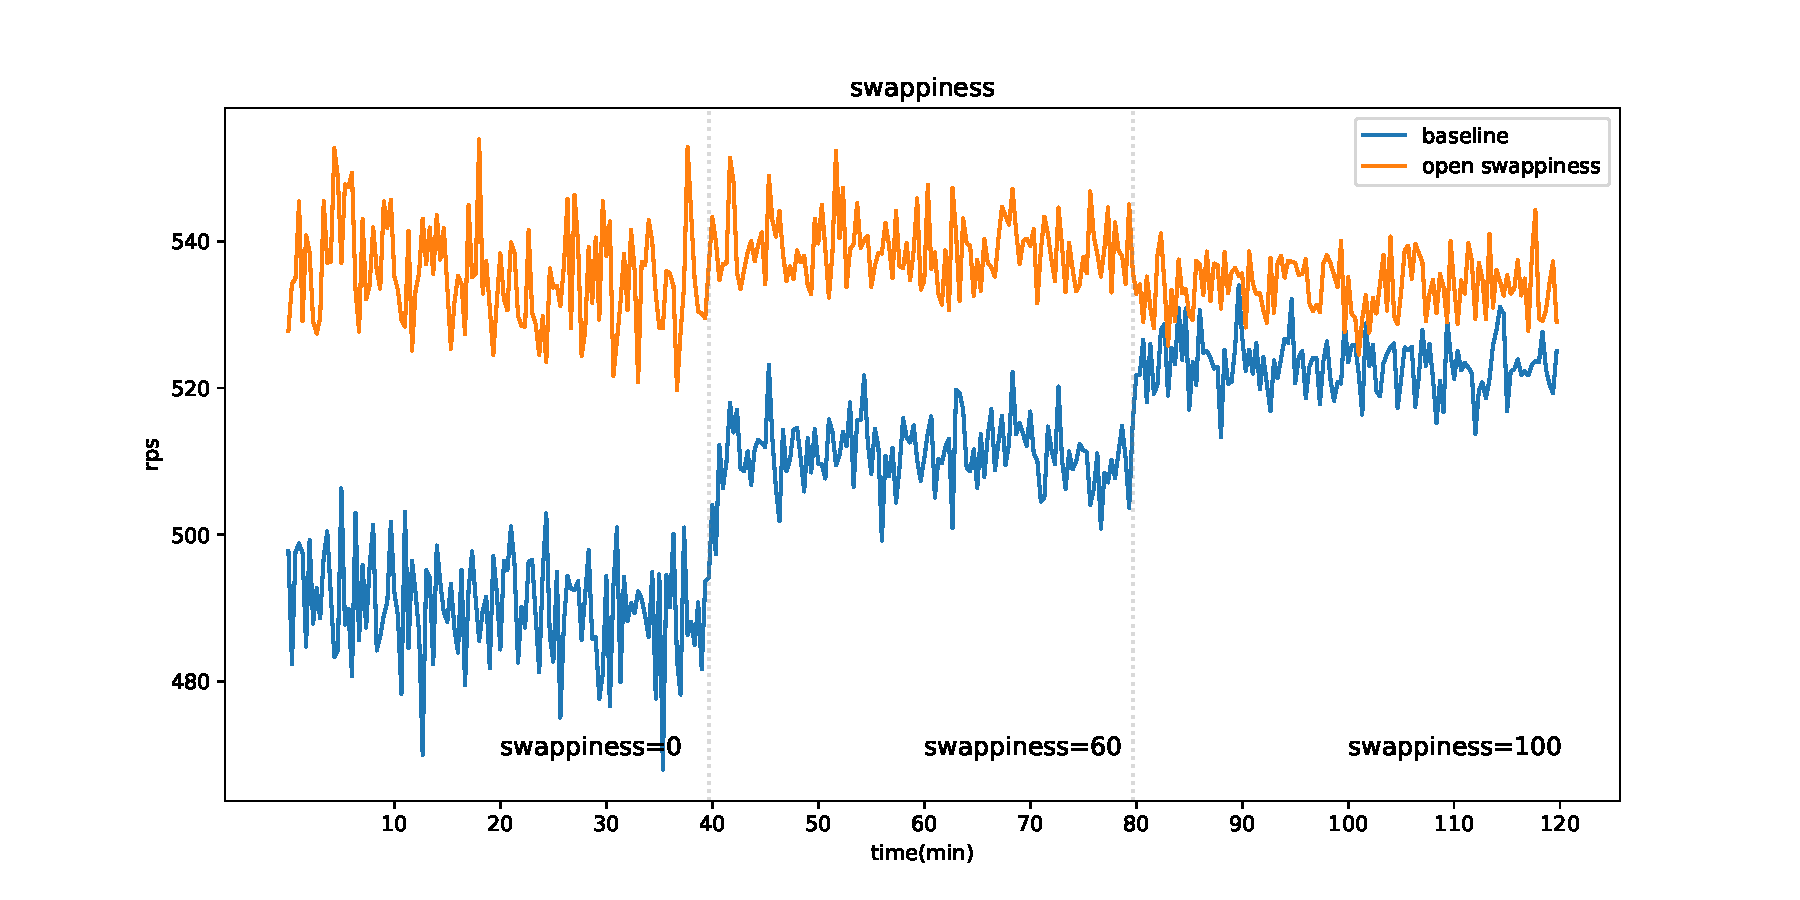
\includegraphics[width=\textwidth,keepaspectratio]{swappiness.pdf}
    \caption{Web Server 在不同  swappiness  下的性能变化}
    \label{fig:web_server_swappiness}
\end{figure}

首先在文件密集型负载(Web Server)下进行测试,如图\ref{fig:web_server_swappiness}所示。在默认内核策略下,当 \(swappiness=0\) 时,系统优先回收文件页而保留匿名页,导致Web Server所需的文件缓存被频繁驱逐,平均RPS仅维持在490左右;当 \(swappiness=60\) 时,系统开始更均衡地回收文件页和匿名页,使得Web Server的关键文件缓存得到一定保留,RPS明显提升至约515;进一步将 \(swappiness\) 提高到100时,RPS继续小幅上升至520左右,但增幅已不显著,这表明在文件密集型负载下,适当提高匿名页回收比例能有效改善系统性能。

当启用自适应均衡算法后,其性能表现更为优异。图中橙色曲线显示,无论 \(swappiness\) 设置为何值,系统吞吐量均维持在535-540之间的较高水平,且波动较小。特别是在 \(swappiness =0\) 的情况下,相比默认策略提升了约10\%的吞吐量,这证明了算法能够准确识别频繁访问的文件页,并通过动态调整回收策略避免了过度驱逐热文件页的问题。

\begin{figure}[htbp]
    \centering
    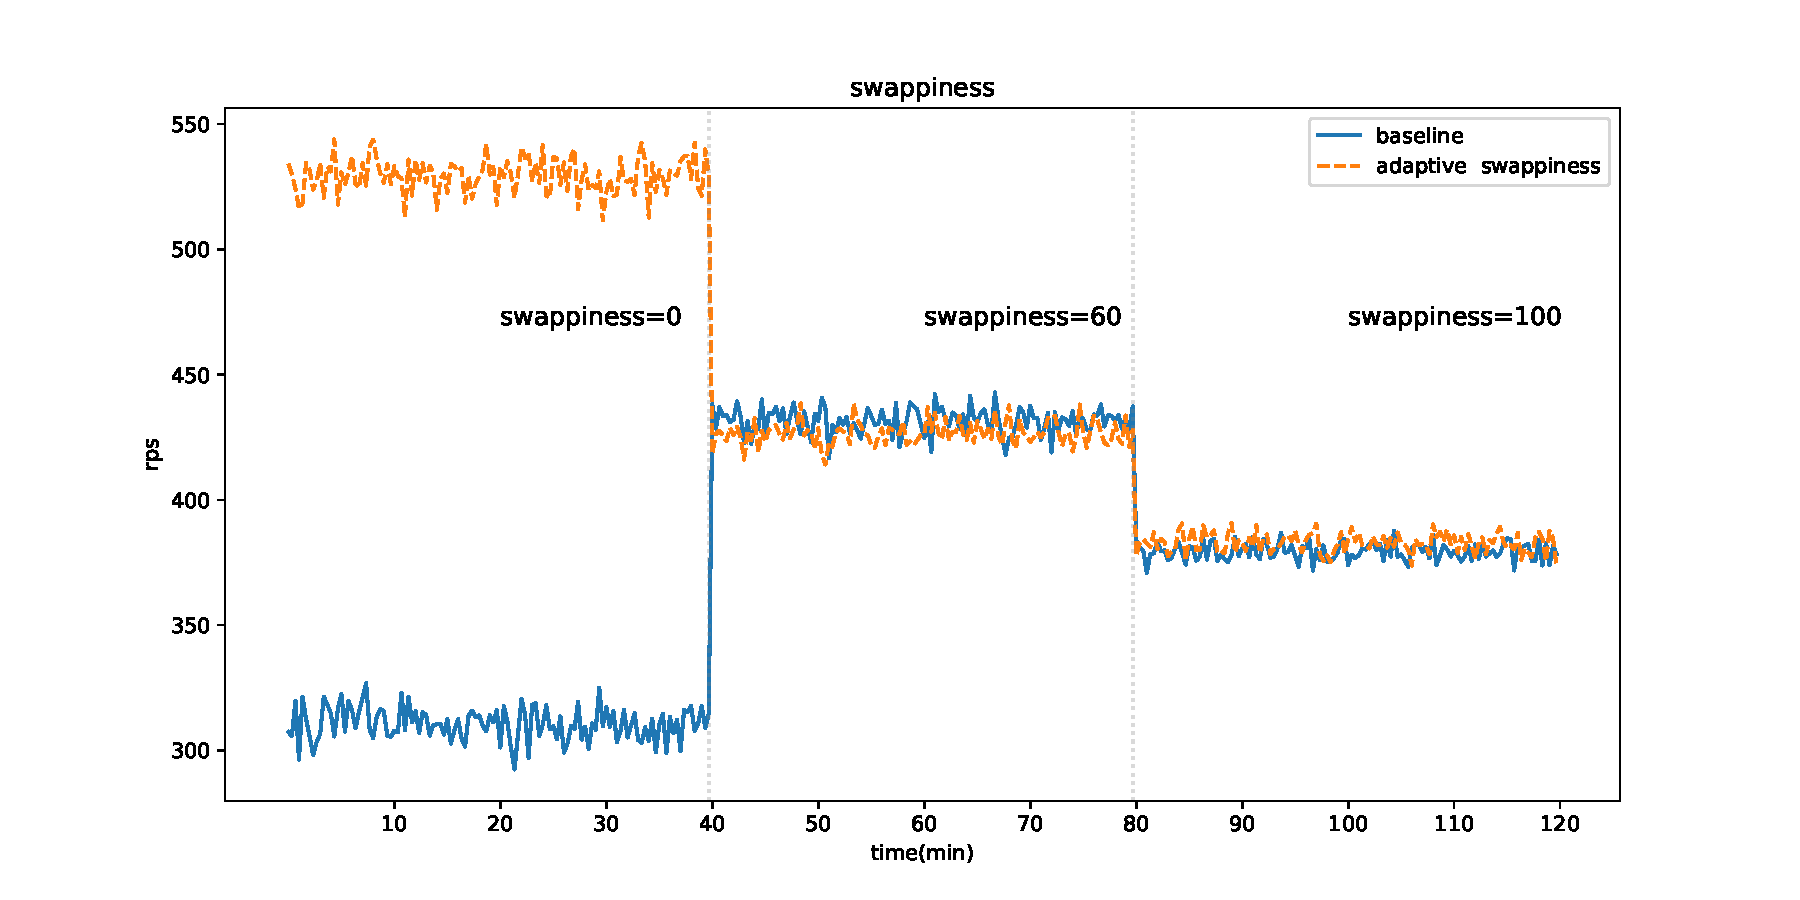
\includegraphics[width=\textwidth,keepaspectratio]{redis_swappiness.pdf}
    \caption{Redis 在不同  swappiness  下的性能变化}
    \label{fig:redis_swappiness}
\end{figure}

为验证算法在不同类型工作负载下的适应性,本文进一步选取了Redis作为内存密集型测试对象。如图\ref{fig:redis_swappiness}所示,Redis测试展现出了与Web Server截然不同的性能特征。在默认内核策略下, \(swappiness =0\) 时Redis的平均RPS仅为310左右;当提高至 \(swappiness =60\) 后,RPS骤增至430左右;而进一步提高至 \(swappiness =100\) 时,性能又下降至380左右。这一曲线变化表明,在匿名页占主导的Redis工作负载中,过低的 \(swappiness\) 值会导致系统几乎不回收匿名页,使得内存压力集中在文件页上,而这些文件页可能包含程序代码等关键部分;适度提高 \(swappiness\) 可以实现更均衡的回收策略;但过高的值则会导致过度回收匿名页从而引发频繁的页面换入换出。

当启用自适应均衡算法后,系统表现出更强的环境适应能力。在 \(swappiness =0\) 的配置下,启用算法的Redis性能(约525 RPS)显著优于默认策略,远高于任何 \(swappiness\) 值下的默认策略表现。这表明算法能够通过分析页面访问模式,自动调整回收策略,避免了在内存紧张时对程序关键文件页的错误驱逐。在 \(swappiness =60\) 和 \(swappiness =100\) 的配置下,启用算法后的性能与默认策略相近,这是因为在Redis这类匿名页占比极高(约90\%)的场景中,文件页缺页率相对较低,算法优化空间有限。

实验结果表明,本文提出的文件页与匿名页均衡算法在不同类型的工作负载下均能展现良好适应性。在文件密集型负载中,算法能够通过精确识别热文件页并保留它们来提升性能;在内存密集型负载中,算法也能避免关键文件页被错误驱逐。虽然在极高匿名页占比的环境中算法的优化空间相对有限,但这也符合内存管理的理论预期,因为当工作集几乎完全由匿名页构成时,页面类型差异化回收的影响自然会降低。通过这两类代表性应用的实验,初步验证了该算法具有较强的通用适应能力。

\section{综合测试}

\subsection{测试目标}

上述实验分别验证了内存压力模块在不同后端介质下的量化能力,以及文件页与匿名页均衡算法在不同类型工作负载下的适应性。为了更深入地了解将二者结合起来后对系统整体性能和资源使用的影响,本文设计了综合测试。该测试主要聚焦以下问题:在持续提供服务的高负载场景下,若开启自适应算法并在不同后端(SSD 与 ZRAM)进行内存卸载,系统能否稳定提升吞吐量并节约内存占用;在用户态应用(如 Web Server)长期占用大规模文件页以及针对容器化的多进程场景下,算法是否依旧有良好的适应性。

\subsection{测试方案}

实验在Web Server场景下,通过预热阶段将高频访问文件页预加载至内存,随后基于第\ref{sec:pressure_based_model}节所述的内存压力动态控制模型,设置0.01的内存压力阈值以触发主动内存卸载。实验采用渐进式压力注入策略,在维持高并发请求的同时,系统性地评估以下四种配置场景的性能表现:(1) 禁用swap机制;(2) 启用SSD作为swap设备;(3) 启用ZRAM作为swap设备;(4) 在场景(2)和(3)基础上,集成自适应算法(包含内存压力监测模块、文件页与匿名页均衡机制以及基于压力的工作集评估策略)。为量化性能差异,本研究重点监测并分析系统吞吐量(RPS)、内存使用率、缺页中断频率(refault)以及p90响应时间等关键性能指标,通过时序数据变化趋势对系统整体性能进行深入分析。

\subsection{实验结果与分析}
\label{sec:test_result}
本研究采用系统吞吐量、内存使用率、缺页中断频率、p90事务响应时间以及容器内存使用效率等关键性能指标,对实验结果进行了系统性评估。图\ref{fig:rps}、图\ref{fig:mem}、图\ref{fig:refault}、图\ref{fig:p90}和图\ref{fig:container_memory}分别展示了各指标的实验结果及其分析。

\subsubsection{系统吞吐量分析}
\begin{figure}[htbp]
    \centering
    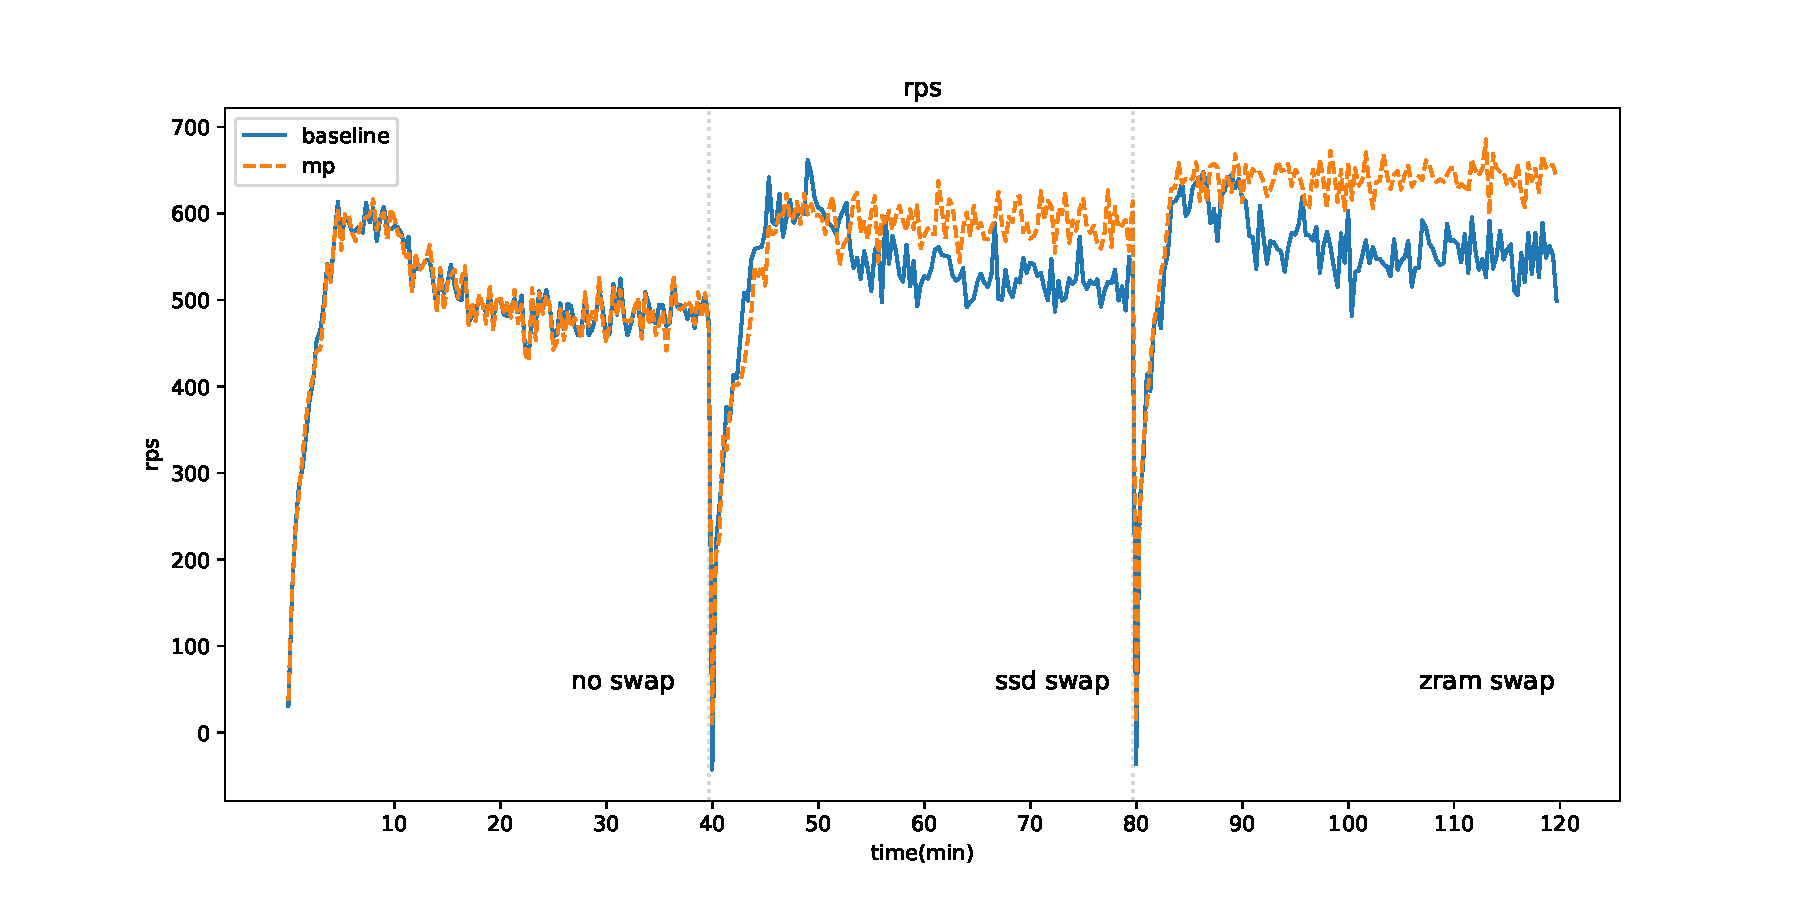
\includegraphics[width=\textwidth,keepaspectratio]{rps.pdf}
    \caption{Web Server 负载在多种场景下的 RPS 对比}
    \label{fig:rps}
\end{figure}
图\ref{fig:rps}展示了Web服务器在不同内存管理策略下的RPS对比情况。实验分为三个独立阶段:无swap(0-40分钟)、SSD交换(40-80分钟)和ZRAM交换(80-120分钟),每个阶段均对比了基准配置与内存压力感知的自适应回收算法(在本节后续简称为 mp 算法)的性能表现。

实验结果表明:
\begin{itemize}
    \item 在无swap阶段,由于内存资源受限,两种配置均出现性能下降趋势,mp算法未表现出显著优势
    \item 在SSD交换阶段,mp算法维持了更稳定且更高的处理能力(平均$580$ RPS),较基准配置(平均$520$ RPS)提升约11.5\%
    \item 在ZRAM交换阶段,mp算法的性能优势进一步扩大,维持在$630$ RPS左右,较基准配置($550$ RPS)提升约14.5\%
\end{itemize}

值得注意的是,mp算法在不同后端场景下的性能提升存在差异:ZRAM场景下提升最为显著,SSD场景下相对较小。这一现象表明,在后端访问成本较低时(如ZRAM的压缩解压延迟远低于SSD的I/O延迟),自适应算法的优势更为明显。

\subsubsection{内存使用分析}
\begin{figure}[htbp]
    \centering
    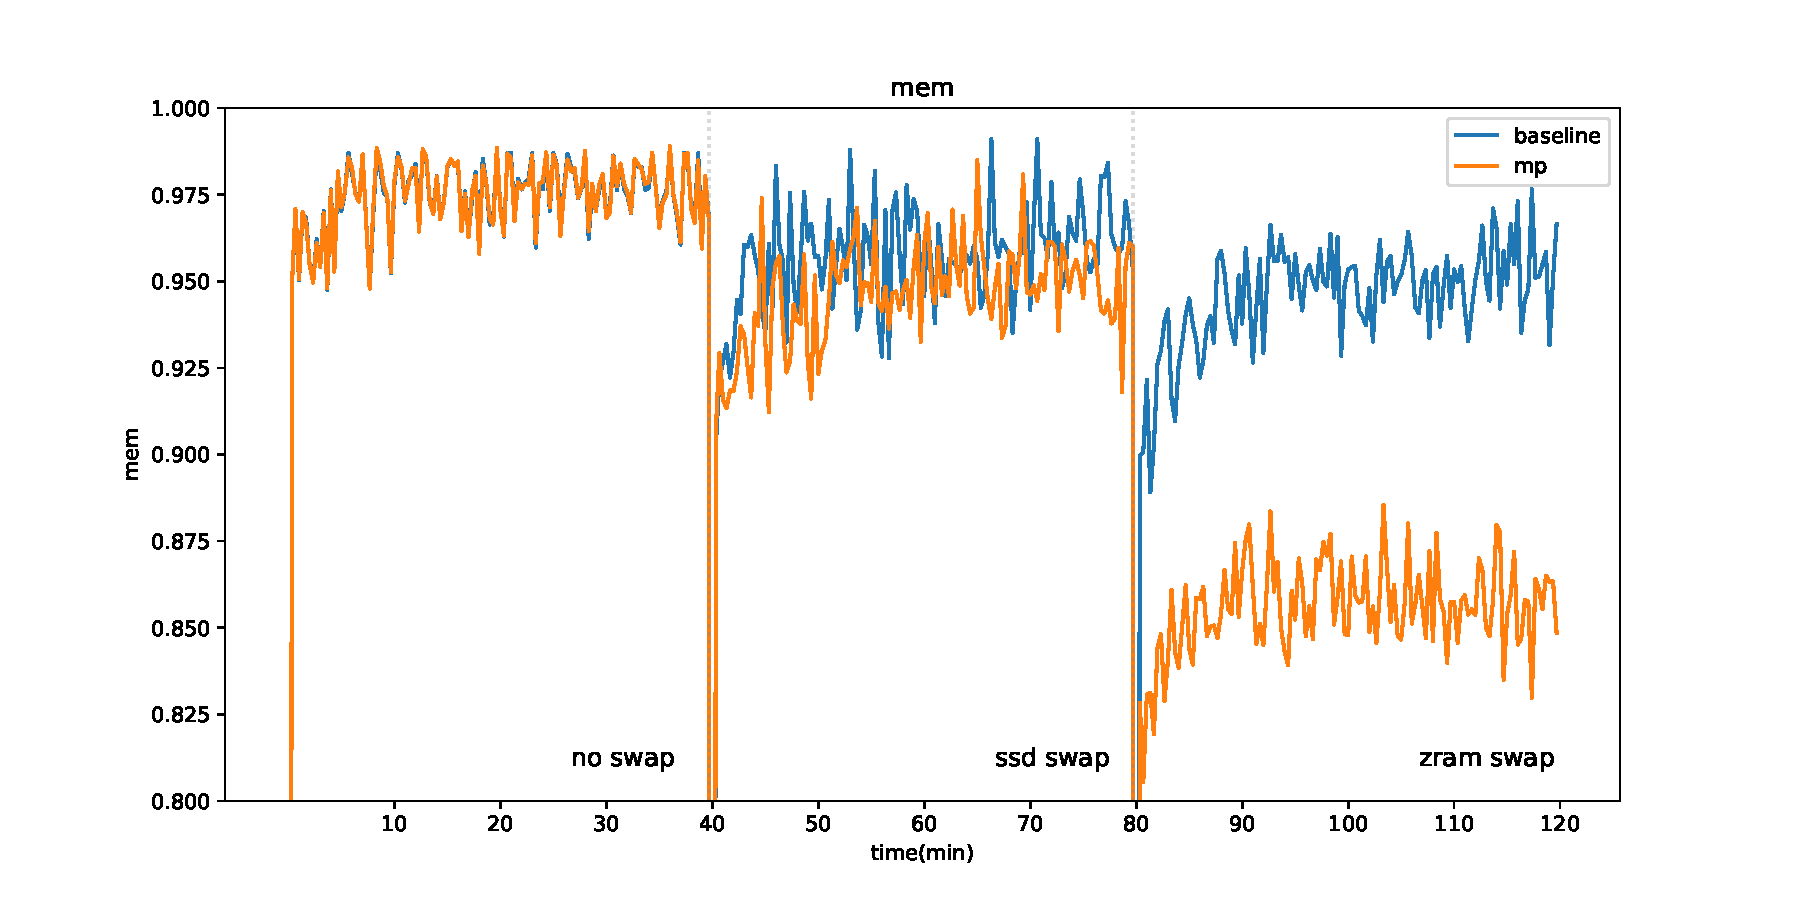
\includegraphics[width=\textwidth,keepaspectratio]{mem.pdf}
    \caption{Web Server 负载在多种场景下的内存使用对比}
    \label{fig:mem}
\end{figure}
图\ref{fig:mem}展示了不同内存管理策略下的实际内存占用情况。实验结果揭示:
\begin{itemize}
    \item 无swap阶段,两种配置均接近内存饱和状态(mp算法:0.97,baseline:略低于0.97)
    \item SSD交换阶段,mp算法与baseline的内存占用率接近(0.94-0.96),未表现出显著差异
    \item ZRAM交换阶段,mp算法的内存占用率(0.94-0.96)显著高于baseline(0.85-0.88),表明mp算法能更有效地识别并卸载低频访问页面
\end{itemize}

内存使用情况与RPS表现相互印证,表明在后端访问成本较低时,mp算法能够更积极地卸载页面,实现更高效的内存资源利用。

\subsubsection{缺页中断分析}
\begin{figure}[htb]
    \centering
    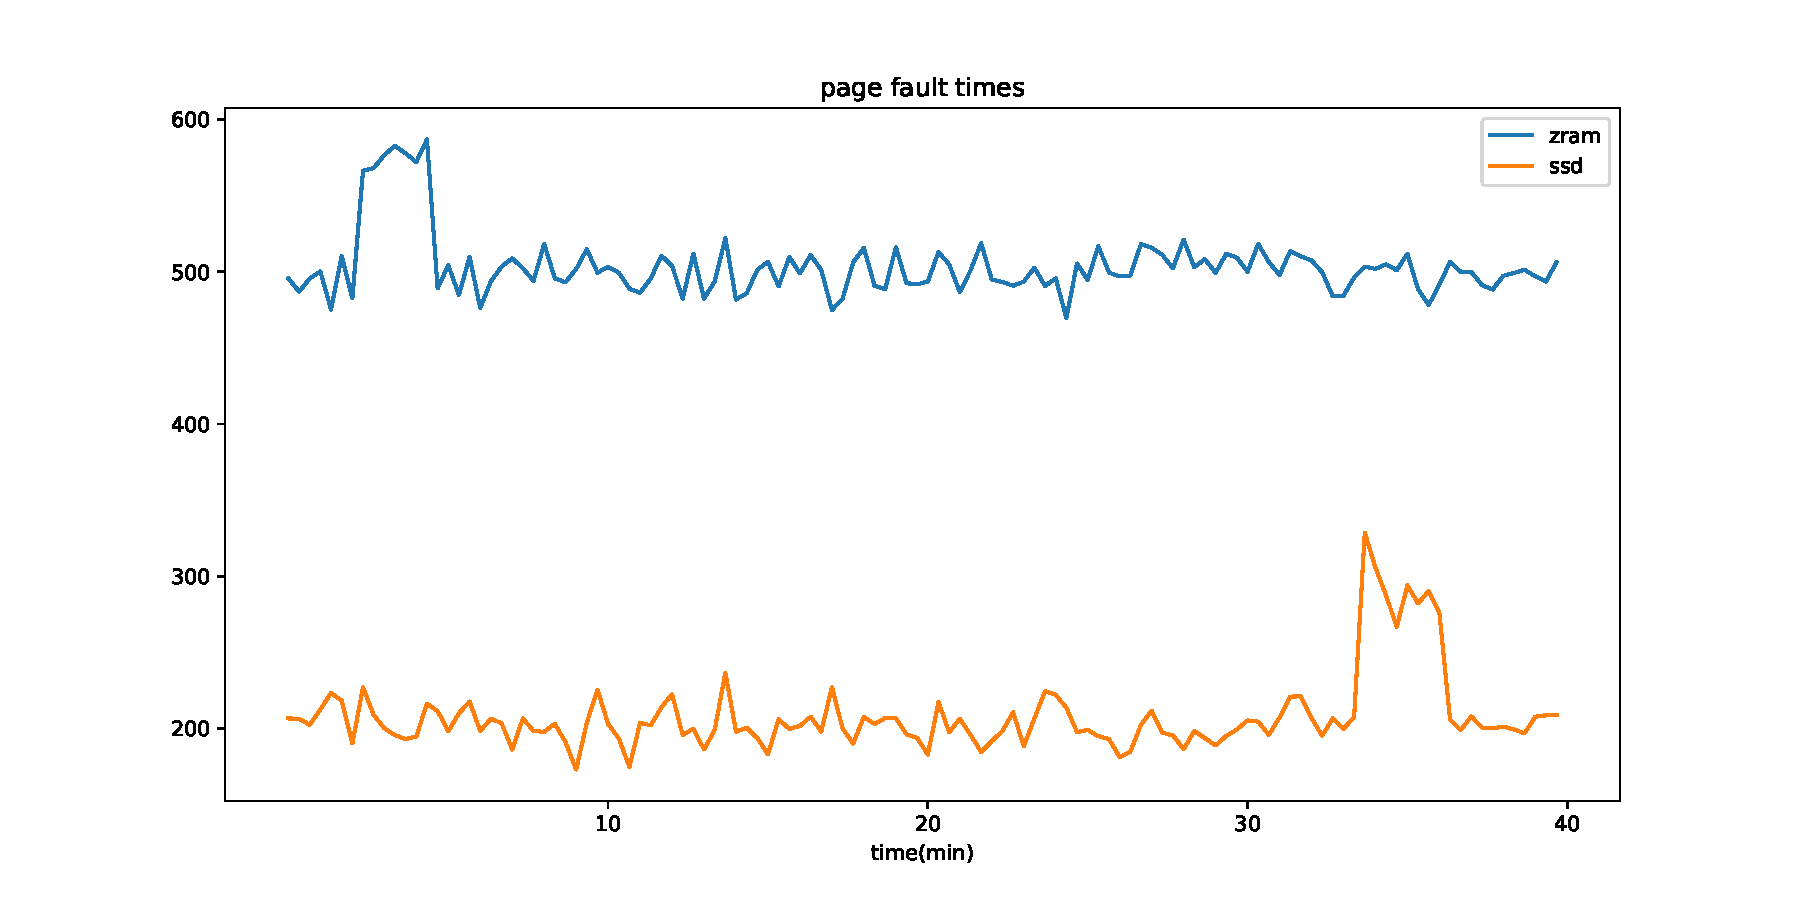
\includegraphics[width=\textwidth,keepaspectratio]{refault.pdf}
    \caption{Web Server 负载在多种场景下的缺页中断次数}
    \label{fig:refault}
\end{figure}
图\ref{fig:refault}展示了两种交换策略下的缺页中断次数对比。实验结果显示:ZRAM策略的缺页中断率显著高于SSD策略。

较高的缺页中断率表明ZRAM策略下内存压力更小,系统能够更积极地卸载内存,这与前述RPS和内存使用情况的分析结果一致。

\subsubsection{响应时间分析}
\begin{figure}[htb]
    \centering
    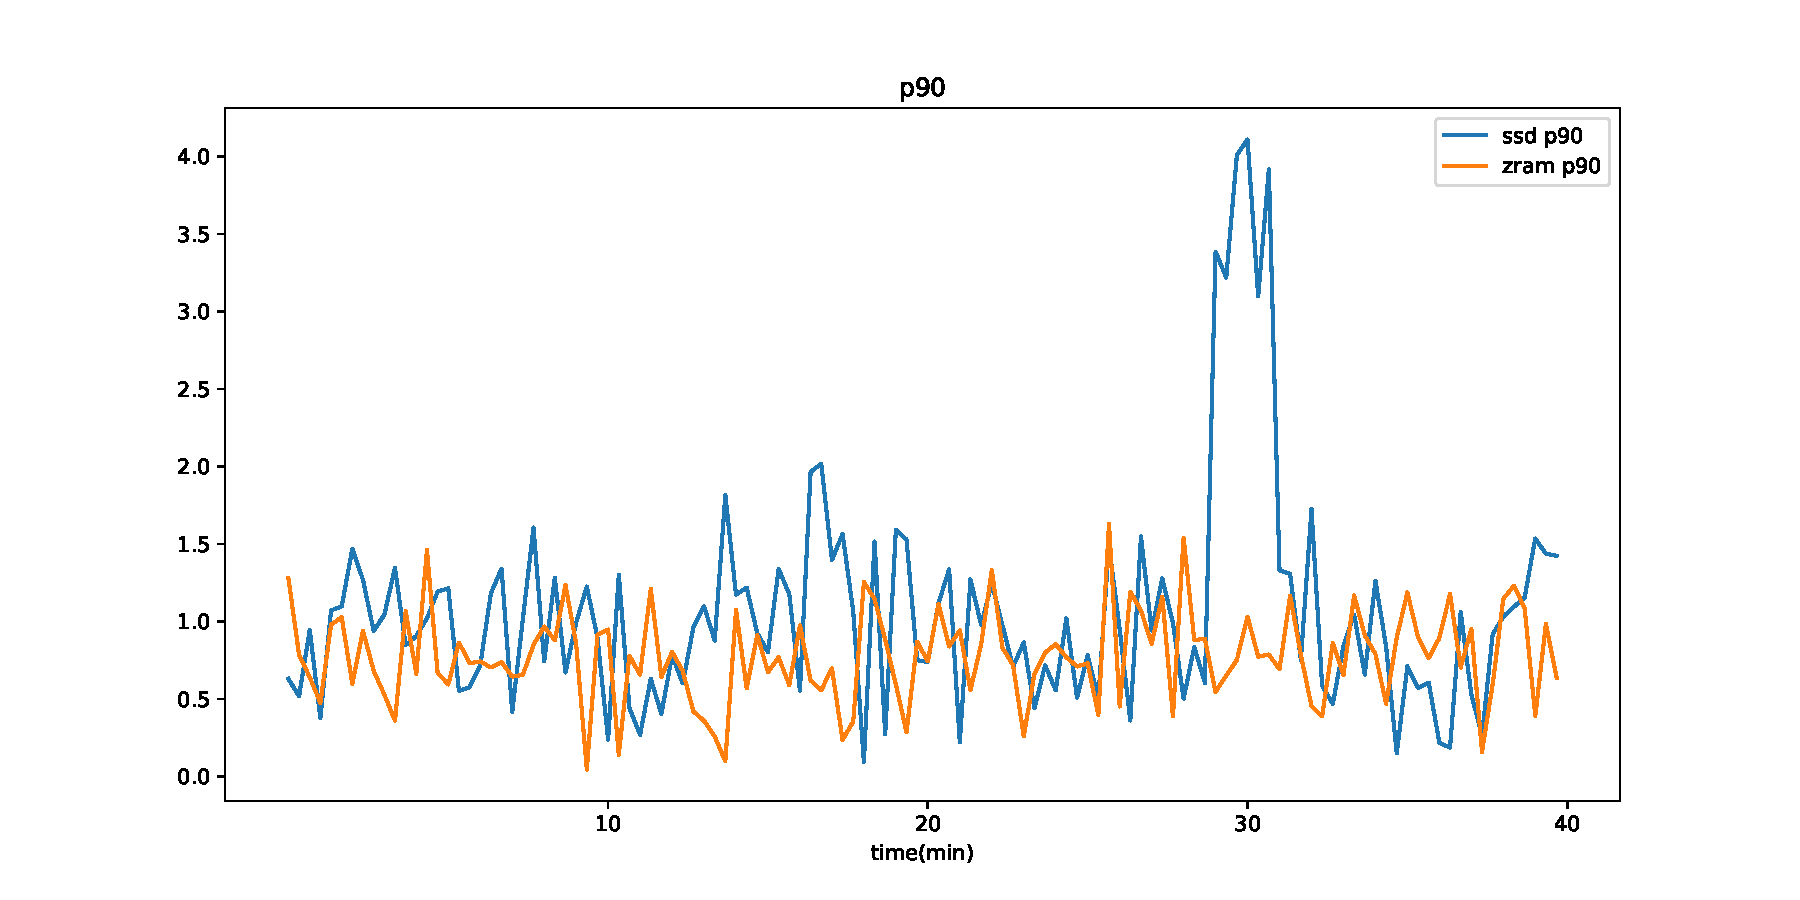
\includegraphics[width=\textwidth,keepaspectratio]{p90.pdf}
    \caption{Web Server 负载在多种场景下的 p90 响应时间对比}
    \label{fig:p90}
\end{figure}
图\ref{fig:p90}展示了不同交换策略下的p90响应时间对比。实验结果表明:
\begin{itemize}
    \item SSD策略的p90响应时间波动性较大,出现多个明显延迟峰值,最高接近4.0
    \item ZRAM策略的p90响应时间普遍维持在较低水平(0.5-1.5),且波动幅度较小
\end{itemize}

这一结果进一步证实了在后端访问成本较低时,系统能够提供更稳定且更低的尾部延迟,从而提升整体服务质量。

\subsubsection{容器内存使用分析}
\begin{figure}[htbp]
    \centering
    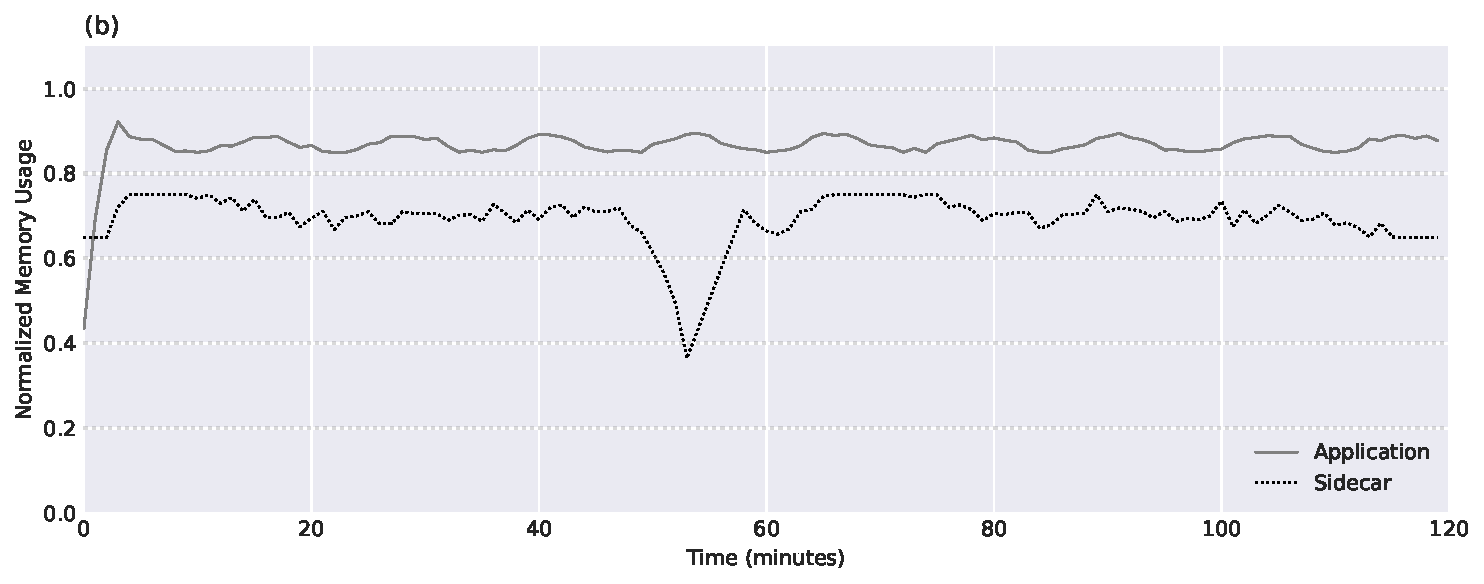
\includegraphics[width=\textwidth,keepaspectratio]{container_memory.pdf}
    \caption{自适应算法在边车容器与业务容器中的内存释放效果对比}
    \label{fig:container_memory}
\end{figure}
图\ref{fig:container_memory}展示了容器化环境下的内存使用情况,其中比较了应用容器(实线)与边车容器(虚线)在 120 分钟观测期内的标准化内存使用率变化。从图中可以观察到以下几个关键特征:
\begin{itemize}
    \item 应用容器的内存使用率(灰色实线)在实验初期迅速上升至约 0.9 左右,并在整个观测期间保持相对稳定,波动范围较小,始终维持在 0.85-0.9 之间。
    \item 边车容器的内存使用率(黑色虚线)总体上明显低于应用容器,大部分时间维持在 0.65-0.75 区间,且波动性更大。特别值得注意的是,在约 50 分钟时刻,边车容器的内存使用率出现了显著下降,一度降至 0.37 左右,随后又迅速恢复。
    \item 两类容器在内存使用模式上呈现明显差异:应用容器内存使用相对刚性且稳定,而边车容器则表现出更强的弹性与波动性。
\end{itemize}

这一结果揭示了边车容器在内存使用特性上的重要发现:边车容器中存在相当比例的低频访问或不活跃页面,这些页面可以被内存压缩或页面回收机制识别并处理。当系统应用内存压力模块与自适应回收算法时,这些低活跃度页面可以有效地被卸载到高性能存储介质(如 ZRAM),从而释放宝贵的物理内存资源。

从图中边车容器内存使用的波动特性可以推断,边车容器相比核心应用容器提供了更多的内存卸载机会。这一发现对于超大规模集群环境具有重要意义:尽管受设备限制无法在本研究中进行大规模集群测试,但可以合理预测,在包含数万甚至数十万容器的生产环境中,针对边车容器的内存优化策略将能够累积显著的内存节省效果。特别是在现代微服务架构中,每个业务容器通常伴随多个边车容器(用于日志收集、监控、流量代理等功能),这些边车容器所产生的虚拟化税会随着集群规模扩大而呈倍数增长。通过对这些边车容器实施有针对性的内存卸载策略,可以有效提高集群整体的内存利用效率,减少因内存压力导致的应用性能下降或 OOM 事件,从而增强系统整体的稳定性与资源使用效率。

\subsubsection{综合分析}
实验结果表明,内存压力感知的自适应回收算法在不同存储后端下均能显著提升系统性能,特别是在高速卸载后端的支持下,其优势更为明显。该算法能够有效缓解内存压力导致的性能波动问题,为Web服务器提供更稳定且更高的请求处理能力。在容器化环境中,边车容器相比应用容器表现出更强的内存使用弹性,为内存优化提供了更多可能性。这些发现为设计面向内存受限环境的高性能系统提供了重要参考。


\section{本章小结}

通过本章一系列实验,可以得出以下主要结论:首先,本文所设计的内存压力模块能够在机械硬盘、SSD 和 ZRAM 这三种卸载后端下有效量化系统的内存压力。其次,文件页与匿名页均衡算法在文件密集型负载中均展现出良好的适用性,其针对 \(swappiness\)  的动态调节可避免过度回收缓存文件页或引发过度的匿名页换入换出,从而在不同场景里带来显著性能增益。再次,在综合测试中,结合内存压力与自适应均衡的整体方案能够高效地释放物理内存并在高负载时保持稳定的吞吐和延迟表现,其中 ZRAM 作为卸载后端时展现了更加出色的性能。最后,在容器化场景下,边车容器的内存占用常常在实际部署中造成可观的资源浪费,通过在内核中实施基于压力的自适应回收机制,能够大幅降低这部分“虚拟化税”,在大规模服务环境下具有突出的应用价值。上述结论为下一步在更复杂或更大规模生产环境中推广这一内存回收与卸载方案提供了重要参考依据。
